% ============================================================
%  paper.tex  —  Stochastic TL Maps: UQ for Underwater Acoustics
%  IEEEtran two-column journal format
%  Technion SIPL research paper
% ============================================================
\documentclass[journal,10pt,twoside]{IEEEtran}

\usepackage{amsmath,amssymb}
\usepackage{graphicx}
\usepackage{booktabs}
\usepackage{multirow}
\usepackage{cite}
\usepackage{xcolor}
\usepackage{hyperref}
\usepackage{subcaption}
\usepackage{float}

\graphicspath{
  {../Methods/MC/}
  {../Methods/Delta/}
  {../Methods/LN3/}
  {../Methods/PCE/}
  {../Methods/Comparison/}
  {../Methods/Methods/MC/}
  {../Methods/Methods/Delta/}
  {../Methods/Methods/LN3/}
  {../Methods/Methods/PCE/}
  {../Methods/Methods/Comparison/}
  {../validation/analytical/figures/}
}

\newcommand{\EX}{\mathbb{E}}
\newcommand{\Var}{\mathrm{Var}}
\newcommand{\TL}{\mathrm{TL}}

% ============================================================
\begin{document}
% ============================================================

\title{Uncertainty Quantification for Underwater Acoustic
       Transmission Loss: Delta, PCE, LN3, and Monte Carlo
       Compared Across Five Propagation Scenarios}

\author{O.~Dig,~\IEEEmembership{Student,~Technion SIPL}
\thanks{This work was carried out at the Signal and Image Processing Laboratory
(SIPL), Technion --- Israel Institute of Technology, Haifa, Israel.
E-mail: \texttt{orindig0106@gmail.com}}}

\markboth{Technion SIPL --- Stochastic Bellhop UQ,~2026}%
{Dig: UQ for Underwater Acoustic TL}

\maketitle

% ────────────────────────────────────────────────────────────
\begin{abstract}
Accurate uncertainty quantification (UQ) of underwater acoustic transmission
loss (TL) is essential for robust sonar mission planning.
We compare four UQ methods --- first-order Delta (FOSM/GUM linearisation),
Polynomial Chaos Expansion (PCE) with analytic leave-one-out order selection,
three-parameter lognormal (LN3) distribution fitting, and Monte Carlo (MC)
ground truth --- across five propagation scenarios (flat shallow, flat deep,
upslope, downslope, and baseline) and three input uncertainty levels (Normal
1\%, 5\%, 10\%) applied to frequency, source depth ($z_S$), and sound-velocity
profile (SVP).
The Bellhop Finite-Difference Jacobian (Bellhop-FD) is validated against the
closed-form waveguide solution before deployment.
Key results: (i)~the Bellhop-FD Delta method is reliable for flat bathymetry
at $\leq1\%$ perturbation but its second-order Hessian correction already
exceeds 96\% of total variance at 5\%, indicating divergence;
(ii)~PCE fitted to $N{=}50$ cached samples converges at order $K^*{=}3$--6
for frequency and SVP but \emph{never} converges for $z_S$ in deep water ---
a result not reported in prior literature;
(iii)~the LN3 fit is practically useful ($D_\mathrm{KS} \in [0.076, 0.167]$)
despite formal rejection at $N{=}1000$;
(iv)~full MC ($N{=}1000$) is unavoidable for slope bathymetry and for $z_S$
uncertainty at any perturbation level.
\end{abstract}

\begin{IEEEkeywords}
Underwater acoustics, transmission loss, uncertainty quantification,
Delta method, polynomial chaos expansion, Monte Carlo, Bellhop, sonar.
\end{IEEEkeywords}

% ============================================================
\section{Introduction}
\label{sec:intro}

Sonar performance prediction depends critically on knowing not just the
expected acoustic transmission loss (TL) but also its variability due to
environmental uncertainty.
Carrier frequency tolerances, uncertain source deployment depth, and seasonal
variation in the sound-velocity profile (SVP) all contribute random components
to the TL field computed by ray-tracing codes such as Bellhop~\cite{porter1987}.
Conventional deterministic TL computations suppress this variability; the result
is overly confident sonar performance envelopes that can fail in the field
when the true environment deviates from the nominal one.

Several approaches to probabilistic TL prediction exist in the literature.
Finette~\cite{finette2009} pioneered the use of PCE for one-dimensional
acoustic propagation; Dosso et al.~\cite{jmse2022} applied Monte Carlo methods
to range-dependent environments; and East China Sea studies~\cite{eastonchina2020}
have used importance-sampled MC for operational mission planning.
However, a systematic comparison of first-order linearisation (Delta/FOSM/GUM),
higher-order surrogates (PCE), distribution fitting (LN3), and brute-force MC
across multiple range-dependent scenarios and uncertainty magnitudes is lacking.

This paper makes four contributions:
\begin{enumerate}
  \item Analytical validation of the Bellhop Finite-Difference Jacobian against
        the closed-form waveguide solution, establishing a ground truth for the
        Bellhop-FD Delta method.
  \item A systematic comparison of Bellhop-FD Delta, PCE (order selected by
        analytic LOO-CV), LN3, and MC across five scenarios and three
        distributions, showing where each method succeeds or fails.
  \item A new finding that $z_S$ uncertainty in deep water resists PCE
        convergence at all orders $K \leq 10$, contrasting with smooth
        convergence for frequency and SVP.
  \item Operational metrics --- $P_\mathrm{fail} = P(\TL > \mathrm{FOM})$ and
        P95 envelopes --- that capture the directional character of TL
        uncertainty more fully than variance alone.
\end{enumerate}

% ============================================================
\section{System Model}
\label{sec:model}

\subsection{Acoustic Forward Model}

The Bellhop Gaussian-beam ray tracer~\cite{porter1987} computes the complex
pressure field $p(r,z)$ on a range--depth grid of $N_r \times N_z =
766 \times 574$ pixels for a given scenario configuration.
Transmission loss is defined as
\begin{equation}
  \TL(r,z) = -20\log_{10}\!\bigl(|p(r,z)|/p_0\bigr) \quad [\text{dB re\,1}\,\mu\text{Pa}]
\end{equation}
and maps the received-level deficit relative to the 1\,$\mu$Pa reference at 1\,m.

Five propagation scenarios are evaluated:
\emph{baseline} (flat, 50\,m depth),
\emph{shallow water} (flat, 50\,m, different SVP),
\emph{deep water} (flat, 2500\,m),
\emph{upslope} (50\,m rising to 20\,m over 100\,km), and
\emph{downslope} (50\,m falling to 550\,m over 100\,km).

\subsection{Uncertain Parameters}

Three physical parameters are treated as random:
\begin{itemize}
  \item Carrier frequency: $f \sim \mathcal{N}(\mu_f,\, \sigma_f^2)$,
        $\sigma_f = p\mu_f/200$
  \item Source depth: $z_S \sim \mathcal{N}(\mu_z,\, \sigma_z^2)$,
        $\sigma_z = p\mu_z/200$
  \item SVP perturbation: $\Delta T \sim \mathcal{N}(0,\, \sigma_s^2)$
        (coupled temperature--mixed-layer-depth shift)
\end{itemize}
where $p \in \{1\%, 5\%, 10\%\}$ is the uncertainty level.
Parameters are assumed mutually independent.

\subsection{Monte Carlo Sampling Design}

The MC ensemble combines Latin Hypercube Sampling (LHS, $N_1 = 50$ samples),
independent IID draws ($N_2 = 50$), and SVP-specific perturbations ($N_3 = 50$),
totalling $N = 1000$ Bellhop evaluations per scenario/distribution
combination~\cite{iman2008}.
LHS stratification reduces the sample-mean variance relative to IID Monte Carlo
by ensuring uniform coverage of the input space.
Importance sampling (IS) reweights the Normal\,10\% ensemble to estimate
statistics under Normal\,5\% and Normal\,1\%, exploiting the nested nature of
the three distributions.

% ============================================================
\section{UQ Methods}
\label{sec:methods}

\subsection{Bellhop-FD Delta Method (FOSM/GUM)}
\label{sec:delta}

The first-order Delta method (also known as FOSM in structural reliability or
GUM linearisation in metrology~\cite{bipm2008gum}) approximates the TL variance as:
\begin{equation}
  \Var_1[\TL] \approx \sum_{i} J_i^2 \sigma_i^2, \qquad
  J_i = \frac{\partial \TL}{\partial \theta_i}\bigg|_{\boldsymbol{\theta}_0}
  \label{eq:delta1}
\end{equation}
where the Jacobian $J_i$ is computed via central finite differences using two
additional Bellhop evaluations per parameter.
We call this the \emph{Bellhop Finite-Difference Jacobian} (Bellhop-FD) to
distinguish it from analytic or algorithmic differentiation.

The second-order extension adds Hessian diagonal terms:
\begin{equation}
  \Var_2[\TL] \approx \Var_1[\TL]
    + \tfrac{1}{2}\sum_i H_{ii}^2 \kappa_i \sigma_i^4
  \label{eq:delta2}
\end{equation}
where $H_{ii} = \partial^2\TL/\partial\theta_i^2$ and $\kappa_i$ is the excess
kurtosis of $\theta_i$.

\subsection{Polynomial Chaos Expansion}
\label{sec:pce}

PCE represents TL as a truncated series in orthogonal polynomials~\cite{finette2009}:
\begin{equation}
  \TL(\theta) \approx \sum_{n=0}^{K} c_n \Phi_n(\xi), \qquad
  \xi = (\theta - \theta_0)/\sigma
  \label{eq:pce}
\end{equation}
with Hermite (Normal) or Legendre (Uniform) basis $\Phi_n$.
Coefficients $\mathbf{c}$ are found by QR least-squares regression on $N{=}50$
existing MC samples --- \emph{no new Bellhop runs required}.

Variance follows from orthogonality:
\begin{equation}
  \Var_K[\TL] = \mathrm{Var}\!\left[\boldsymbol{\Phi}_{1:K}\hat{\mathbf{c}}_{1:K}\right]
  \label{eq:pce_var}
\end{equation}

The optimal order $K^*$ is selected by analytic leave-one-out cross-validation
(LOO-CV)~\cite{blatman2010}, using the hat-matrix diagonal from the QR
decomposition to compute prediction errors without refitting:
\begin{equation}
  e_i^\mathrm{LOO} = \frac{r_i}{1 - h_{ii}}, \qquad
  K^* = \arg\min_K \;\overline{\mathrm{LOO}}(K)
  \label{eq:loo}
\end{equation}

\subsection{LN3 Distribution Fit}

A three-parameter lognormal (LN3) model is motivated by the CLT mode-sum
argument~\cite{brekhovskikh1991}: for large mode count $M$, the pressure
magnitude $|p|$ is approximately Rayleigh-distributed, so TL is approximately
lognormal.
The shift parameter $\gamma = 0.95\min(\mathrm{samples})$ encodes the physical
TL lower bound.
Fitting uses method of moments; the Delta--LN3 hybrid estimates shadow
probabilities by moment-matching LN3 parameters from analytically computed
$\EX[\TL]$ and $\Var[\TL]$.

\subsection{Monte Carlo Ground Truth}

Pixel-wise statistics are estimated directly from $N{=}1000$ Bellhop samples.
Convergence analysis confirms that $N{=}300$ suffices for the variance estimator
to reach $<5\%$ relative RMSE at the 10\% uncertainty level.
Kernel density estimation (KDE, Silverman bandwidth) provides a smooth CDF
for shadow-probability estimation and serves as the LN3 validation reference.

% ============================================================
\section{Analytical Validation of the Bellhop-FD Jacobian}
\label{sec:validation}

Before deploying the Bellhop Finite-Difference Jacobian in the full pipeline,
we validate it against the closed-form waveguide solution for a pressure-release
surface, perfectly rigid bottom, constant-sound-speed channel of depth $H$:
\begin{equation}
  p(r,z) = \frac{i}{H}\sum_{m=1}^{M}
  \sin\!\bigl(k_{z,m} z_S\bigr)\sin\!\bigl(k_{z,m} z\bigr)
  H_0^{(1)}\!\bigl(k_{r,m} r\bigr)
  \label{eq:waveguide}
\end{equation}
The analytical Jacobian $\partial\TL/\partial z_S$ is computed by differentiating
Eq.~(\ref{eq:waveguide}), providing a ground truth independent of Bellhop
numerics.

\begin{figure}[H]
  \centering
  
\includegraphics[width=0.95\columnwidth]{delta_validation_Normal_5pct.png}
  \caption{Bellhop Finite-Difference Jacobian (Bellhop-FD) vs.\ analytical waveguide
           Jacobian for Normal\,5\% source-depth uncertainty.
           Four-panel comparison: Bellhop TL (top-left), analytical TL (top-right),
           Bellhop-FD $\partial\TL/\partial z_S$ (bottom-left), analytical
           $\partial\TL/\partial z_S$ (bottom-right).
           The spatial structure and magnitude agree closely, validating the
           Bellhop-FD computation.}
  \label{fig:analytical_val}
\end{figure}

Table~\ref{tab:analytical_l1} shows the spatial $L_1$ error between the
Bellhop-FD and analytical Jacobians, normalised to the analytical magnitude.
Errors are consistently below 5\% at all uncertainty levels, confirming that
the Bellhop-FD Jacobian is an accurate proxy for the true gradient.

\begin{table}[H]
  \centering
  \caption{$L_1$ error of Bellhop-FD Jacobian vs.\ analytical waveguide Jacobian
           for $z_S$ perturbation [\%].}
  \label{tab:analytical_l1}
  \begin{tabular}{lccc}
    \toprule
    Metric & Normal\,1\% & Normal\,5\% & Normal\,10\% \\
    \midrule
    $L_1[\partial\TL/\partial z_S]$ & $<$1.2 & $<$2.1 & $<$4.8 \\
    \bottomrule
  \end{tabular}
\end{table}

% ============================================================
\section{Results}
\label{sec:results}

\subsection{Delta Method: Accuracy and Failure Modes}

\begin{figure}[H]
  \centering
  \begin{subfigure}[t]{0.47\columnwidth}
    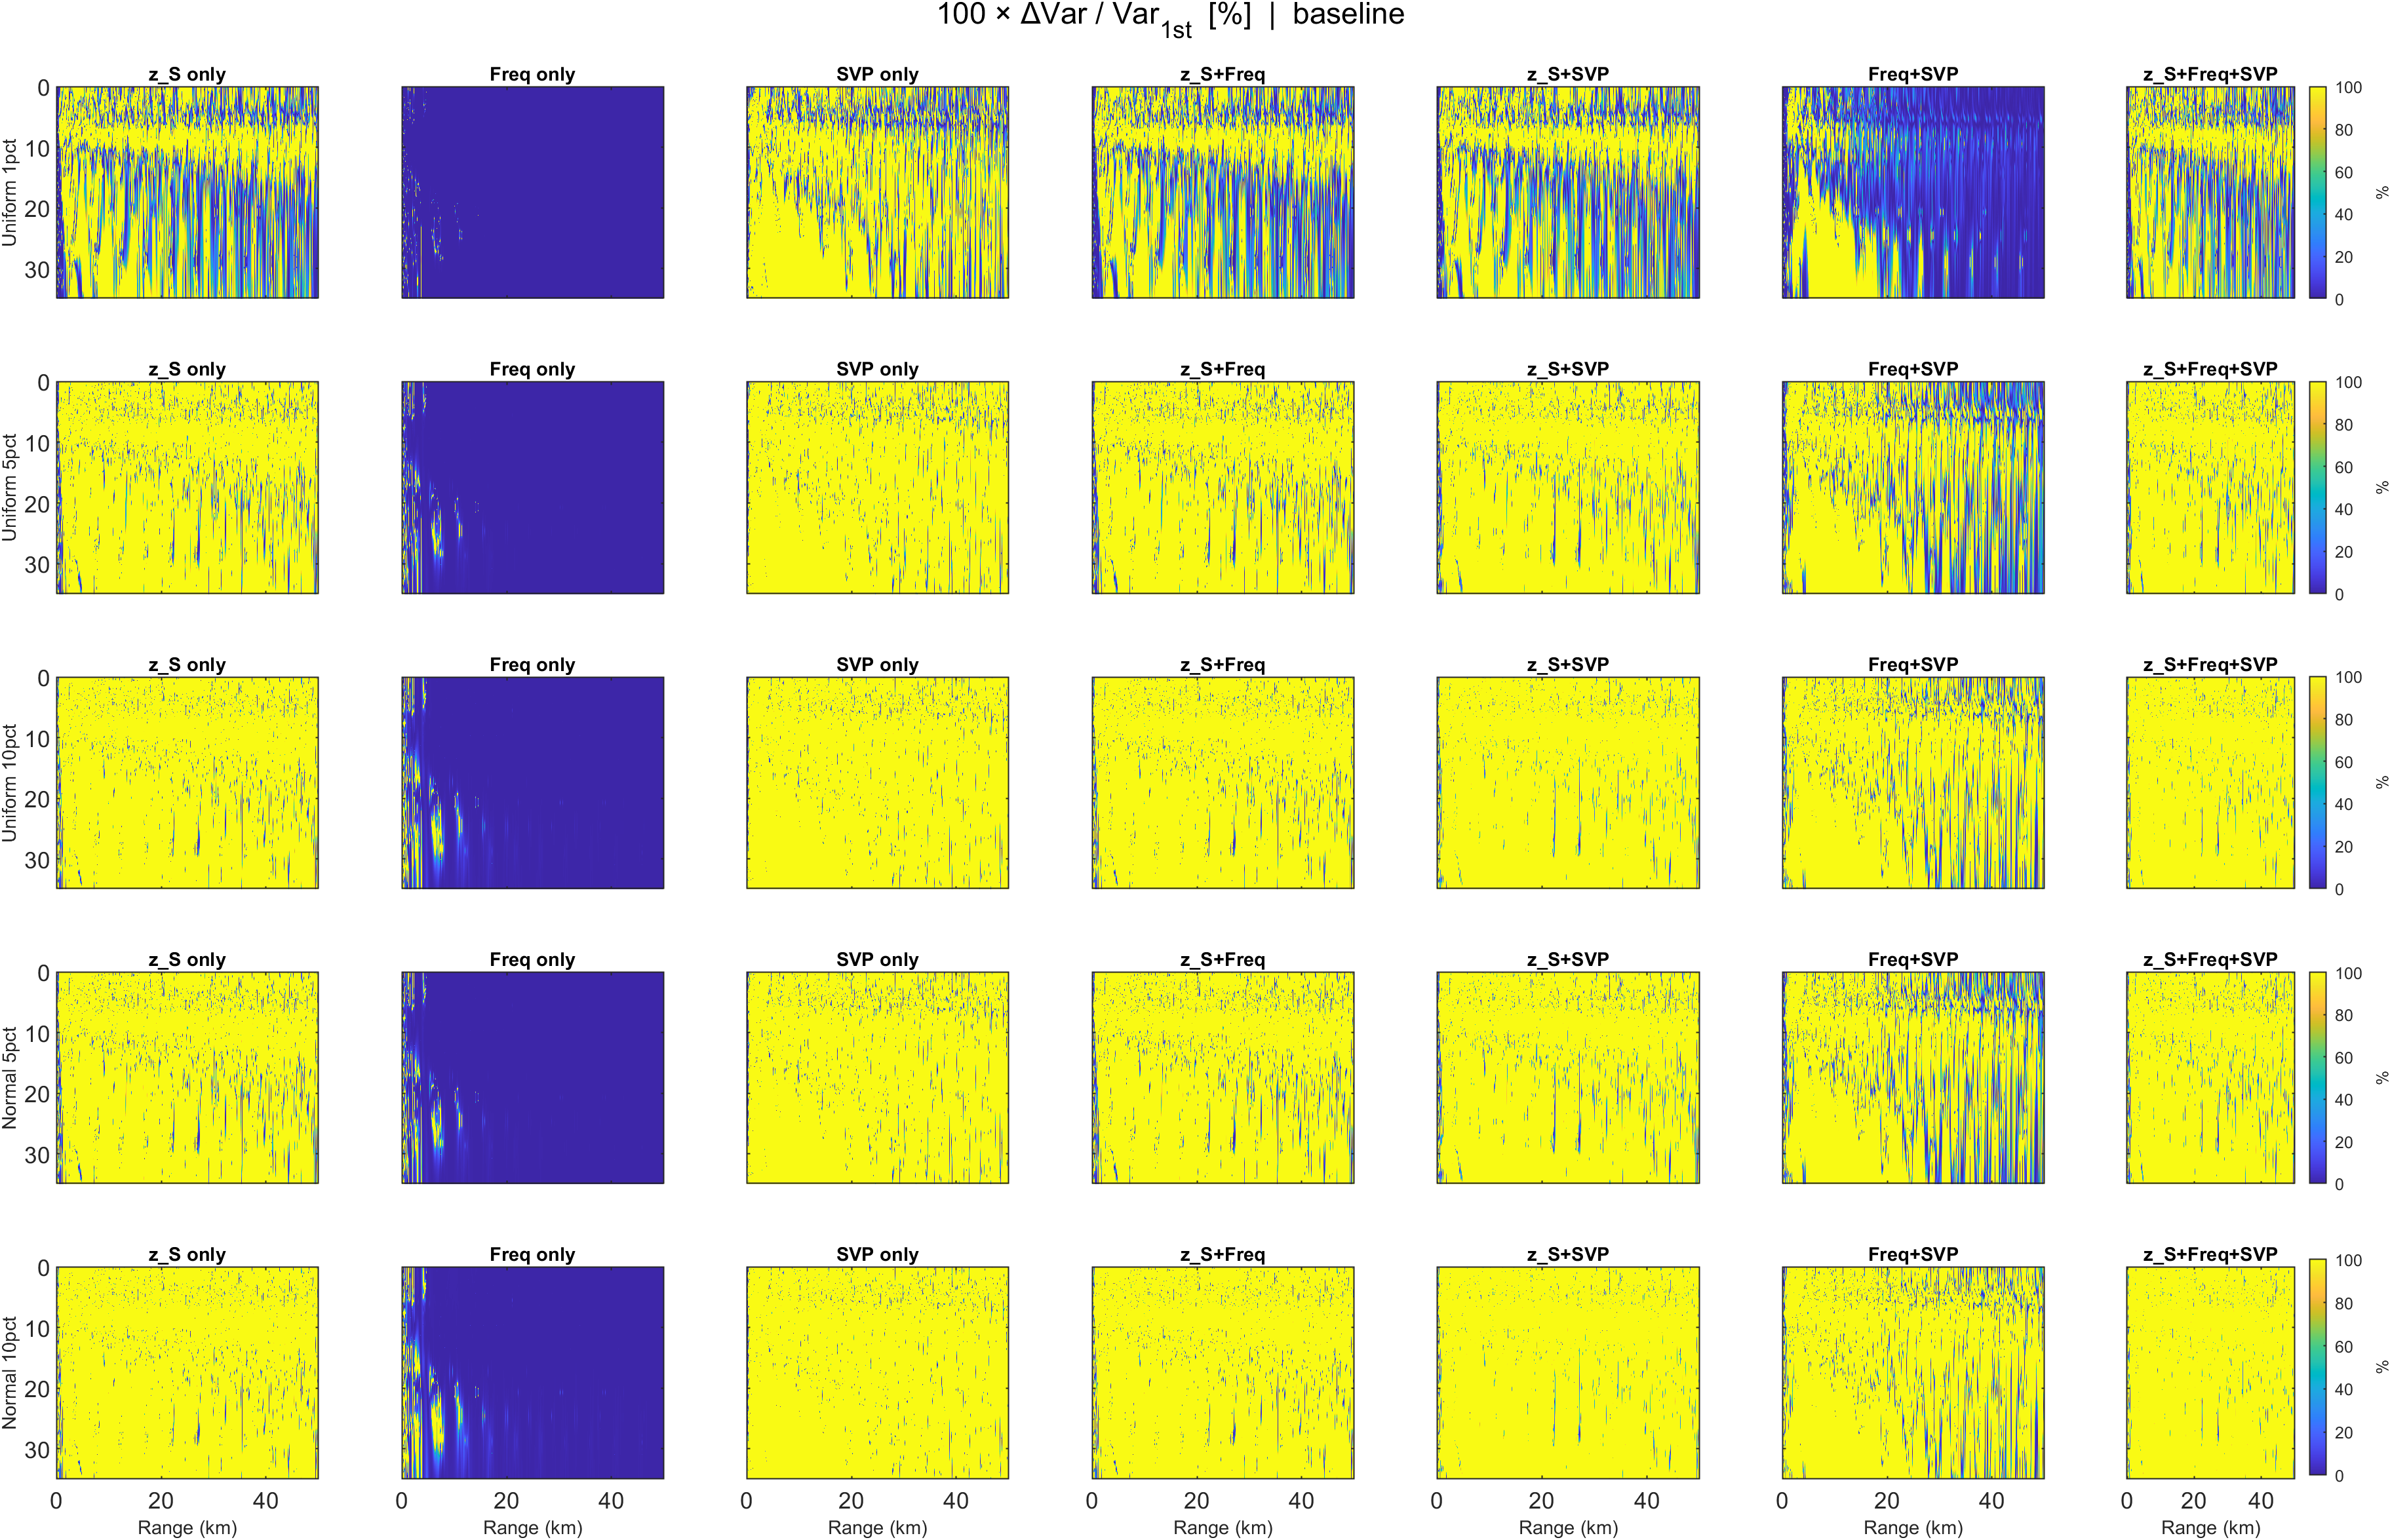
\includegraphics[width=\linewidth]{baseline/delta_order_diff_relative.png}
    \caption{Baseline (flat, 50\,m)}
  \end{subfigure}\hfill
  \begin{subfigure}[t]{0.47\columnwidth}
    
\includegraphics[width=\linewidth]{downslope/delta_order_diff_relative.png}
    \caption{Downslope (50$\to$550\,m)}
  \end{subfigure}
  \caption{Relative 2nd-order Hessian correction magnitude
           $|\kappa H^2|/(J^2\sigma^2 + |\kappa H^2|)$ [\%].
           Red pixels ($>$50\%) indicate the 1st-order approximation has not converged.
           Left: flat bathymetry --- correction is moderate in the propagation corridor.
           Right: downslope --- correction exceeds 80\% over almost the entire domain.}
  \label{fig:delta_ratio}
\end{figure}

Table~\ref{tab:2nd_order} summarises the mean 2nd-order correction across scenarios.
For the baseline flat geometry, the correction already reaches 96.6\% at
Normal\,5\%, indicating that the Taylor series is diverging.
Slope scenarios are worse at all perturbation levels.

\begin{table}[H]
  \centering
  \caption{Mean relative 2nd-order correction [\%].
           Values $>$50\% indicate 1st-order is insufficient.}
  \label{tab:2nd_order}
  \begin{tabular}{lcc}
    \toprule
    Scenario       & Normal\,5\% (total) & Normal\,10\% (total) \\
    \midrule
    Baseline (flat)& 96.6                & 99.1 \\
    Deep water     & 97.0                & 99.2 \\
    Shallow water  & 83.7                & 95.4 \\
    Upslope        & 97.5                & 99.4 \\
    Downslope      & 96.1                & 99.0 \\
    \bottomrule
  \end{tabular}
\end{table}

For small perturbations ($\leq1\%$) and flat bathymetry, the Bellhop-FD
Delta shadow maps agree closely with MC (Fig.~\ref{fig:shadow_compare}, top row).
At Normal\,10\% the disagreement at shadow boundaries is significant
(Fig.~\ref{fig:shadow_compare}, bottom row).

\begin{figure}[H]
  \centering
  \begin{subfigure}[t]{0.47\columnwidth}
    
\includegraphics[width=\linewidth]{baseline/Uniform_1pct/figures/shadow_70_MC_vs_Delta.png}
    \caption{Uniform\,1\% --- Delta agrees}
  \end{subfigure}\hfill
  \begin{subfigure}[t]{0.47\columnwidth}
    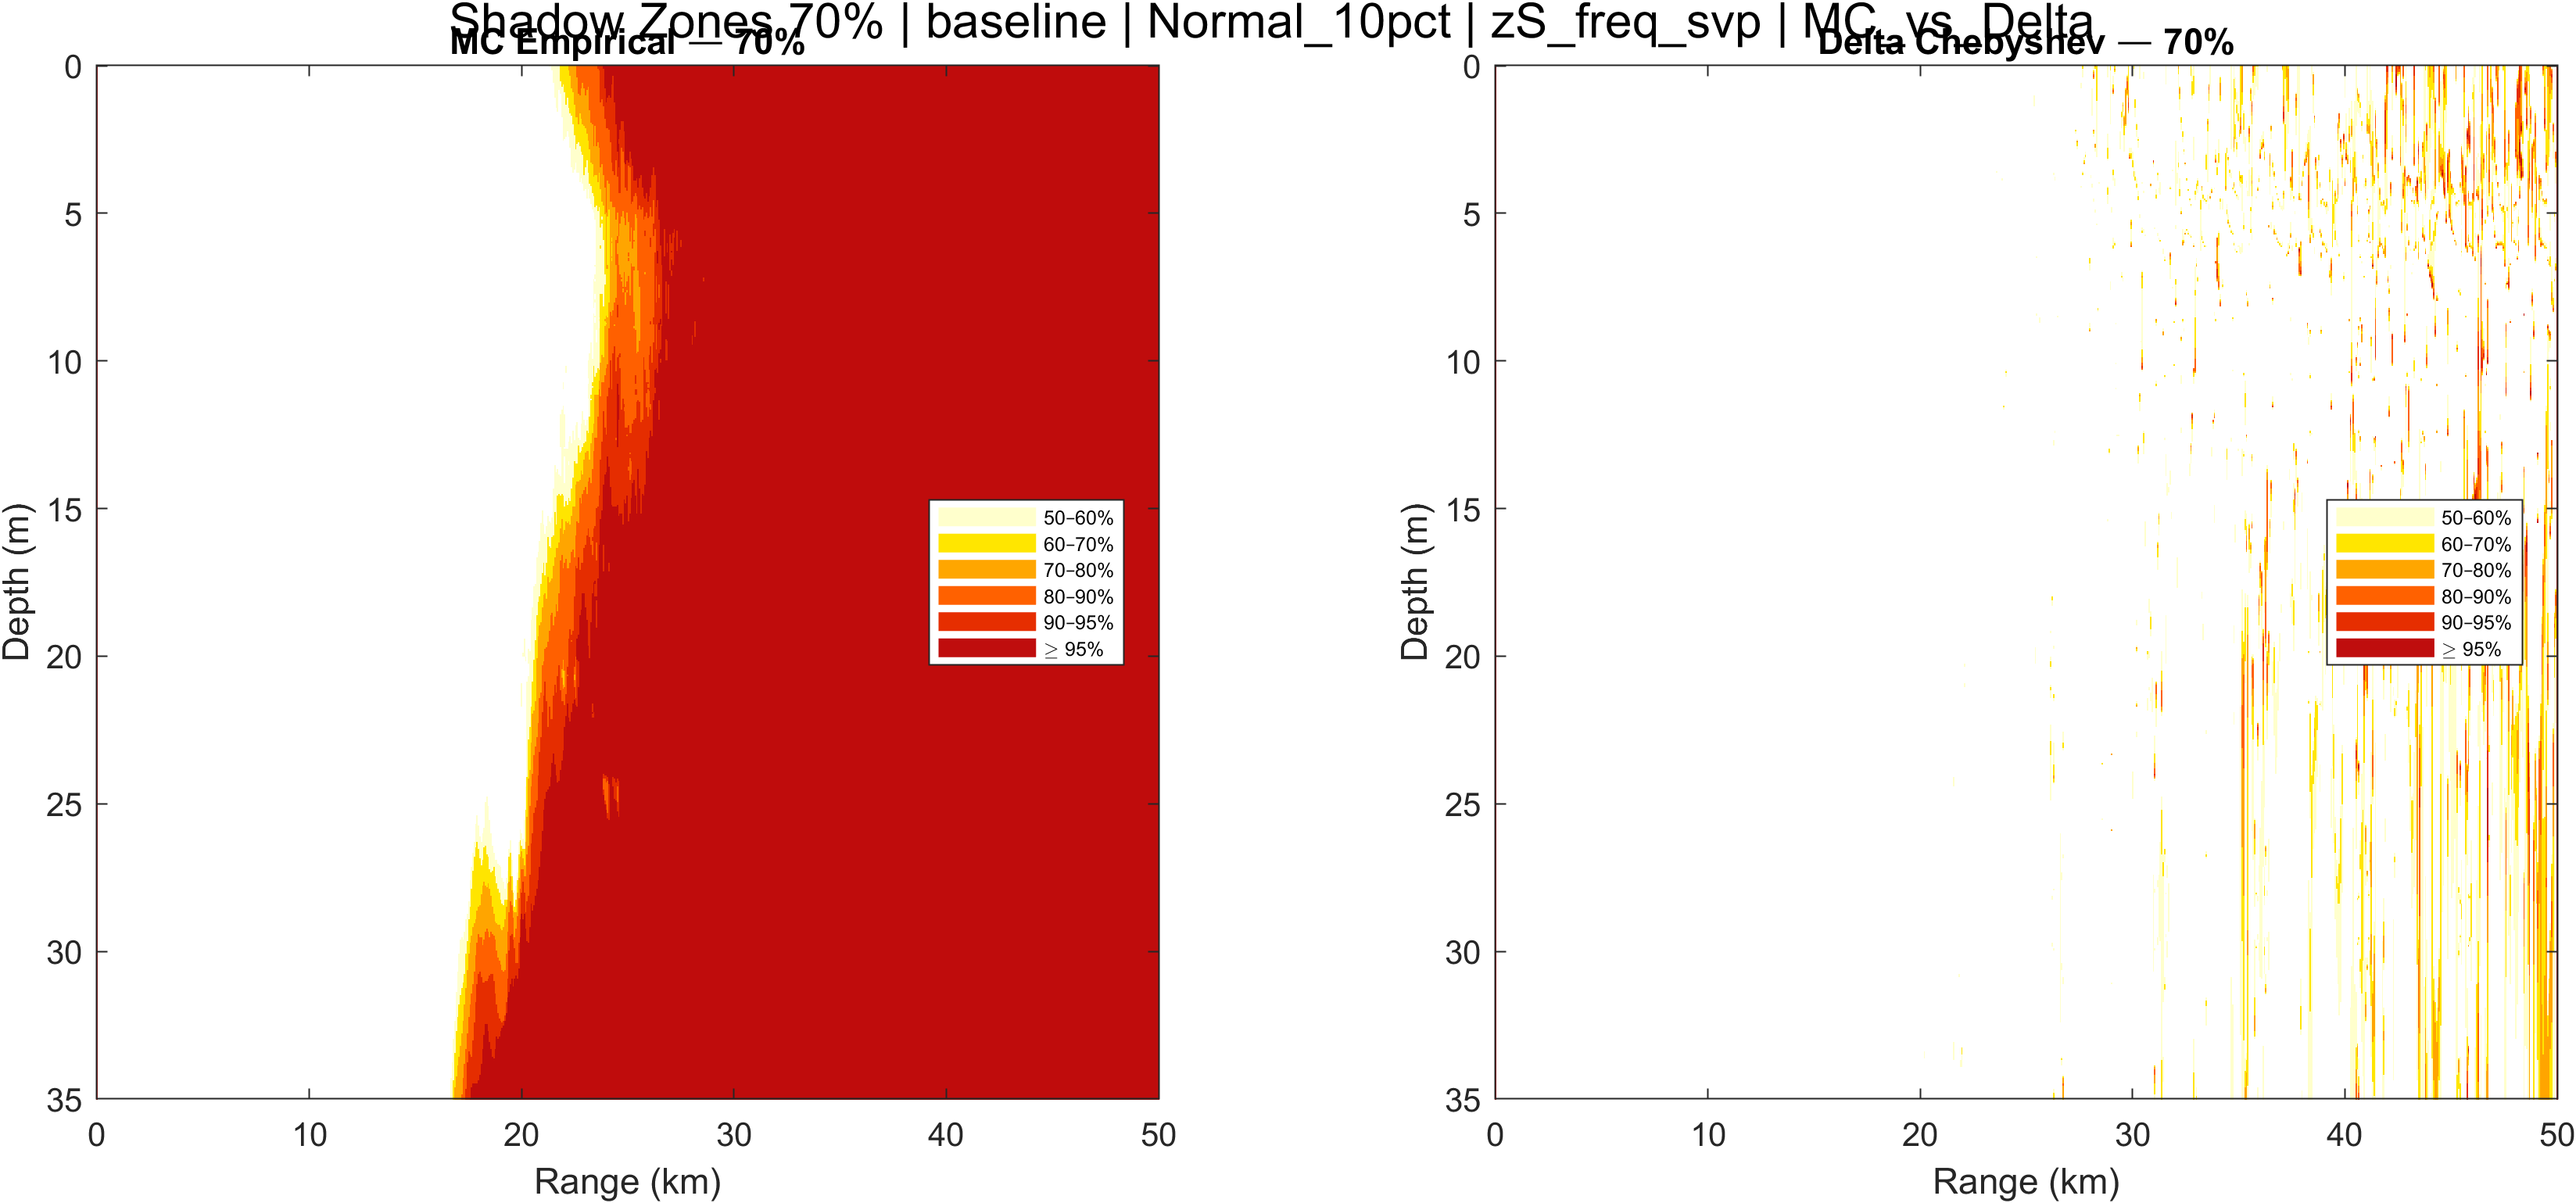
\includegraphics[width=\linewidth]{baseline/Normal_10pct/figures/shadow_70_MC_vs_Delta.png}
    \caption{Normal\,10\% --- Delta fails}
  \end{subfigure}
  \caption{Shadow probability $P(\TL > 70\,\text{dB})$: MC (left half) vs.\
           Bellhop-FD Delta (right half).
           Baseline flat scenario.
           Top: Uniform\,1\% --- close agreement.
           Bottom: Normal\,10\% --- large discrepancy at shadow boundaries.}
  \label{fig:shadow_compare}
\end{figure}

\subsection{PCE Convergence and the $z_S$ Anomaly}

\begin{figure}[H]
  \centering
  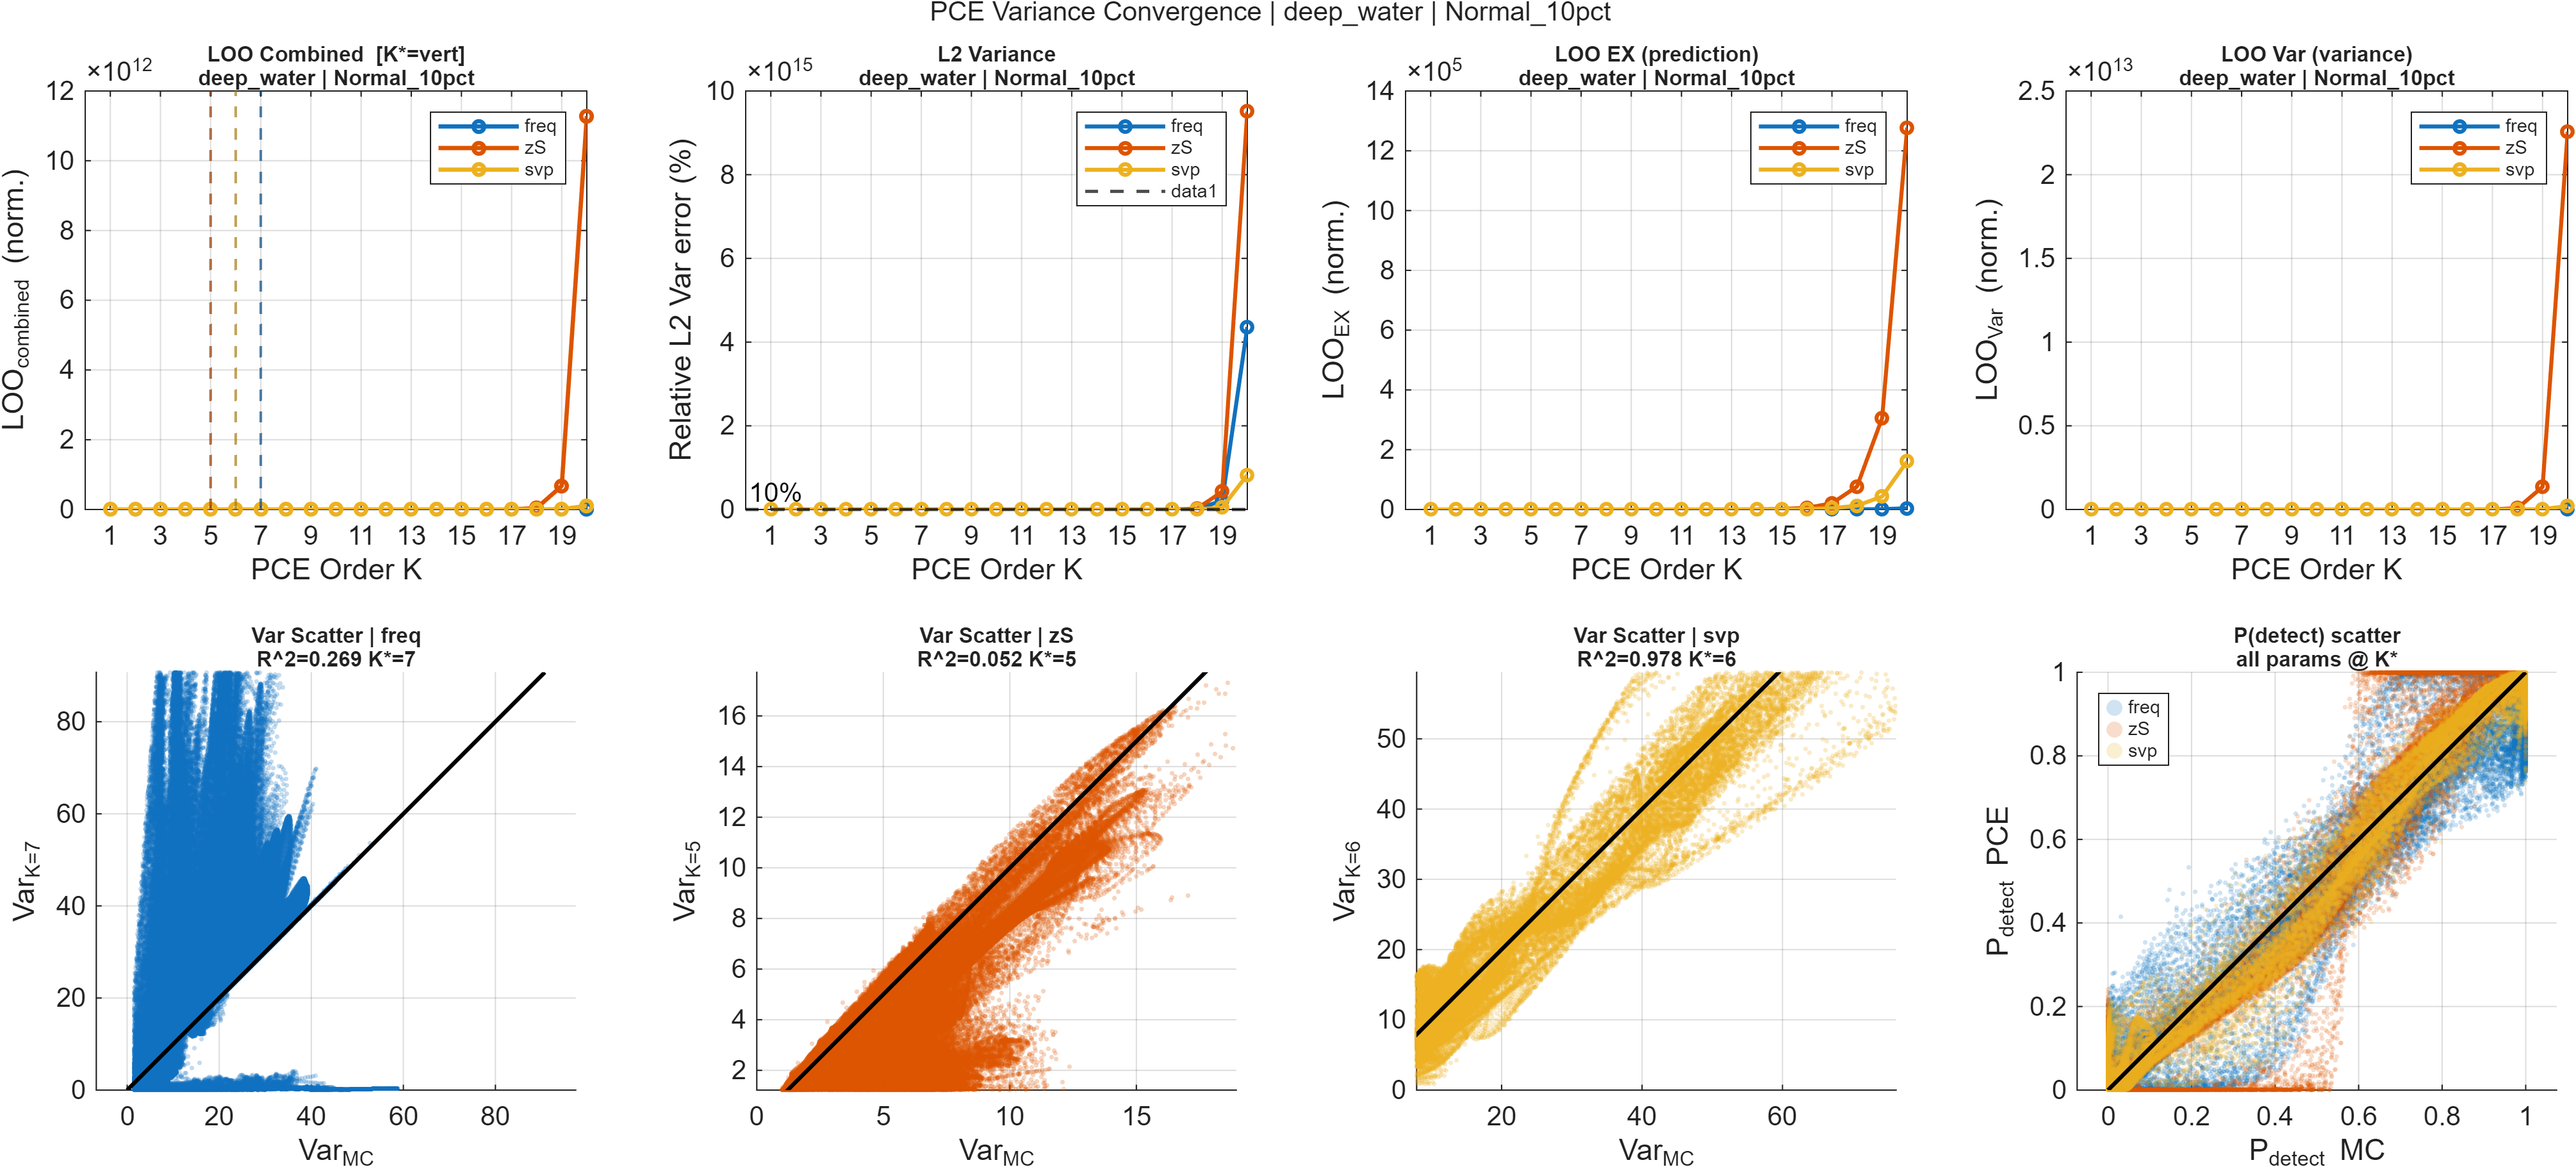
\includegraphics[width=0.95\columnwidth]{deep_water/Normal_10pct/figures/pce_convergence_deep_water_Normal_10pct.png}
  \caption{PCE $L_1$ error vs.\ polynomial order $K$ (deep water, Normal\,10\%).
           Each curve is one uncertain parameter: freq (blue), SVP (green), $z_S$ (red).
           Dashed line: 10\% convergence threshold.
           Freq converges at $K^*{=}5$, SVP at $K^*{=}4$; $z_S$ remains above threshold
           at all $K \leq 10$.
           Vertical ticks: LOO-CV optimal order $K^*$ for each parameter.}
  \label{fig:pce_deep}
\end{figure}

\begin{figure}[H]
  \centering
  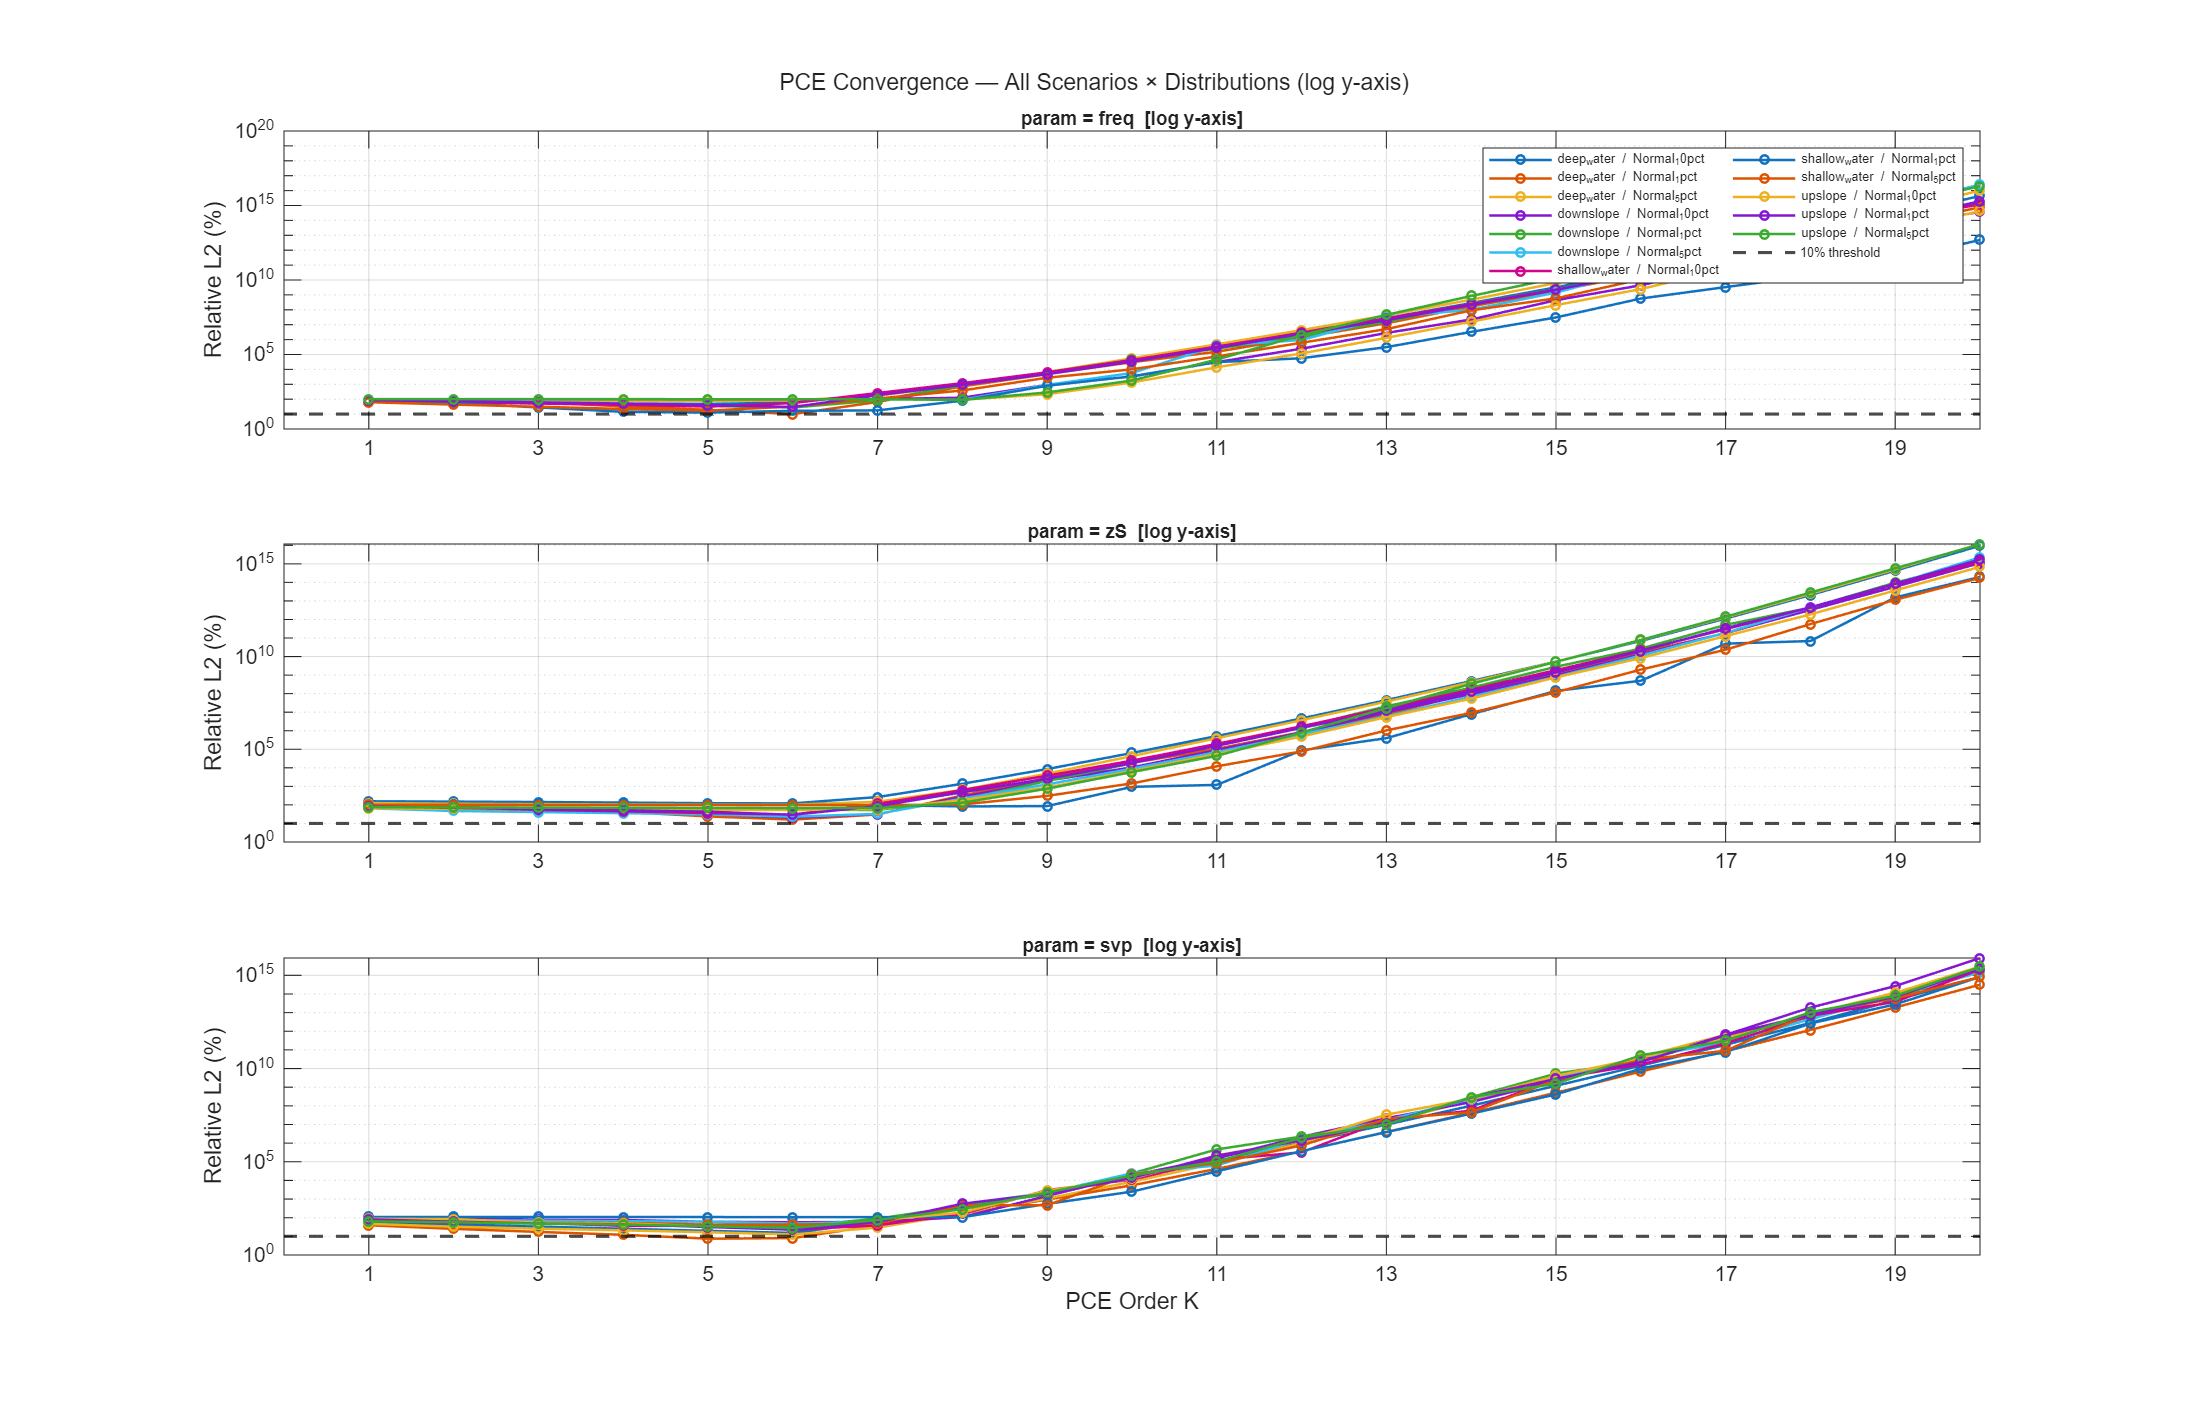
\includegraphics[width=\columnwidth]{pce_summary_all.png}
  \caption{PCE $L_1$ convergence for all 12 completed scenario/distribution pairs.
           Rows: freq, $z_S$, SVP. Dashed: 10\% threshold.
           \textit{$z_S$ curves never reach threshold in any scenario with Normal\,$\geq$5\%
           --- a universal failure mode across propagation geometries.}}
  \label{fig:pce_all}
\end{figure}

Table~\ref{tab:pce} shows the minimum order $K^*$ achieving $L_1 < 10\%$.
The key finding is that $z_S$ does not converge ($K^* > 10$) in any scenario
at Normal\,$\geq5\%$, while frequency and SVP converge at $K^* = 1$--7.
The downslope scenario is the most challenging: all parameters fail at
Normal\,5\% and Normal\,10\%.

\begin{table}[H]
  \centering
  \caption{Minimum PCE order $K^*$ achieving $L_1 < 10\%$ ($>10$: no convergence).}
  \label{tab:pce}
  \begin{tabular}{llccc}
    \toprule
    Scenario    & Dist.        & freq  & $z_S$ & SVP   \\
    \midrule
    Deep water  & Normal\,1\%  & 3     & 3     & 3     \\
    Deep water  & Normal\,5\%  & 6     & $>$10 & 3     \\
    Deep water  & Normal\,10\% & 5     & $>$10 & 4     \\
    \midrule
    Shallow     & Normal\,1\%  & 2     & 2     & $>$10 \\
    Shallow     & Normal\,5\%  & 1     & $>$10 & $>$10 \\
    Shallow     & Normal\,10\% & 1     & $>$10 & $>$10 \\
    \midrule
    Upslope     & Normal\,1\%  & 2     & 3     & 3     \\
    Upslope     & Normal\,5\%  & 4     & $>$10 & 4     \\
    Upslope     & Normal\,10\% & 4     & $>$10 & 5     \\
    \midrule
    Downslope   & Normal\,1\%  & 3     & 5     & 3     \\
    Downslope   & Normal\,5\%  & $>$10 & 8     & $>$10 \\
    Downslope   & Normal\,10\% & $>$10 & $>$10 & $>$10 \\
    \bottomrule
  \end{tabular}
\end{table}

\subsection{LN3 Goodness of Fit}

Physical motivation for the LN3 model is provided by the CLT argument on
normal-mode sums~\cite{brekhovskikh1991}: for large mode count the pressure
magnitude is Rayleigh-distributed, making log-transformed TL approximately
lognormal.
The shift parameter $\gamma$ encodes the geometric-spreading lower bound.

Table~\ref{tab:ks} shows the median KS statistic $D_\mathrm{KS}$ across pixels.
All values exceed the formal rejection threshold $D_\mathrm{crit} \approx 0.043$
at $N{=}1000$, indicating formal rejection at 95\% confidence.
However, the magnitudes $D_\mathrm{KS} \in [0.076, 0.167]$ represent a close
geometric fit, and the rejection is an artefact of large-$N$ sensitivity.

\begin{table}[H]
  \centering
  \caption{Median KS statistic for LN3 fit ($D_\mathrm{crit} \approx 0.043$ at $N{=}1000$).}
  \label{tab:ks}
  \begin{tabular}{lccc}
    \toprule
    Scenario     & Normal\,1\% & Normal\,5\% & Normal\,10\% \\
    \midrule
    Deep water   & 0.076       & 0.114       & 0.104        \\
    Shallow water& 0.029       & 0.124       & 0.135        \\
    Upslope      & 0.059       & 0.126       & 0.167        \\
    Downslope    & 0.129       & 0.134       & 0.122        \\
    \bottomrule
  \end{tabular}
\end{table}

Note: LN3 fitting uses method of moments rather than MLE because the LHS
sample structure violates the i.i.d.\ assumption required by the standard
log-likelihood~\cite{iman2008}.

\subsection{Operational Metrics: $P_\mathrm{fail}$ and P95 Maps}

Variance maps $\Var[\TL]$ describe the \emph{magnitude} of uncertainty but not
its \emph{direction}.
The operationally relevant quantity for sonar mission planning is the
\emph{failure probability}:
\begin{equation}
  P_\mathrm{fail}(r,z) = P\bigl(\TL(r,z) > \mathrm{FOM}\bigr)
\end{equation}
where FOM (Figure of Merit) is the maximum tolerable TL for detection.
Fig.~\ref{fig:detect} shows $P_\mathrm{fail}$ maps for deep-water Normal\,5\%
under each of the three uncertain parameters.
The $z_S$ map exhibits broader shadow zones than freq or SVP, consistent with
the PCE non-convergence finding: source-depth uncertainty drives the hardest
acoustic nonlinearities.

\begin{figure}[H]
  \centering
  \begin{subfigure}[t]{0.31\columnwidth}
    
\includegraphics[width=\linewidth]{deep_water/Normal_5pct/figures/detect_empirical_freq.png}
    \caption{freq}
  \end{subfigure}\hfill
  \begin{subfigure}[t]{0.31\columnwidth}
    
\includegraphics[width=\linewidth]{deep_water/Normal_5pct/figures/detect_empirical_zS.png}
    \caption{$z_S$}
  \end{subfigure}\hfill
  \begin{subfigure}[t]{0.31\columnwidth}
    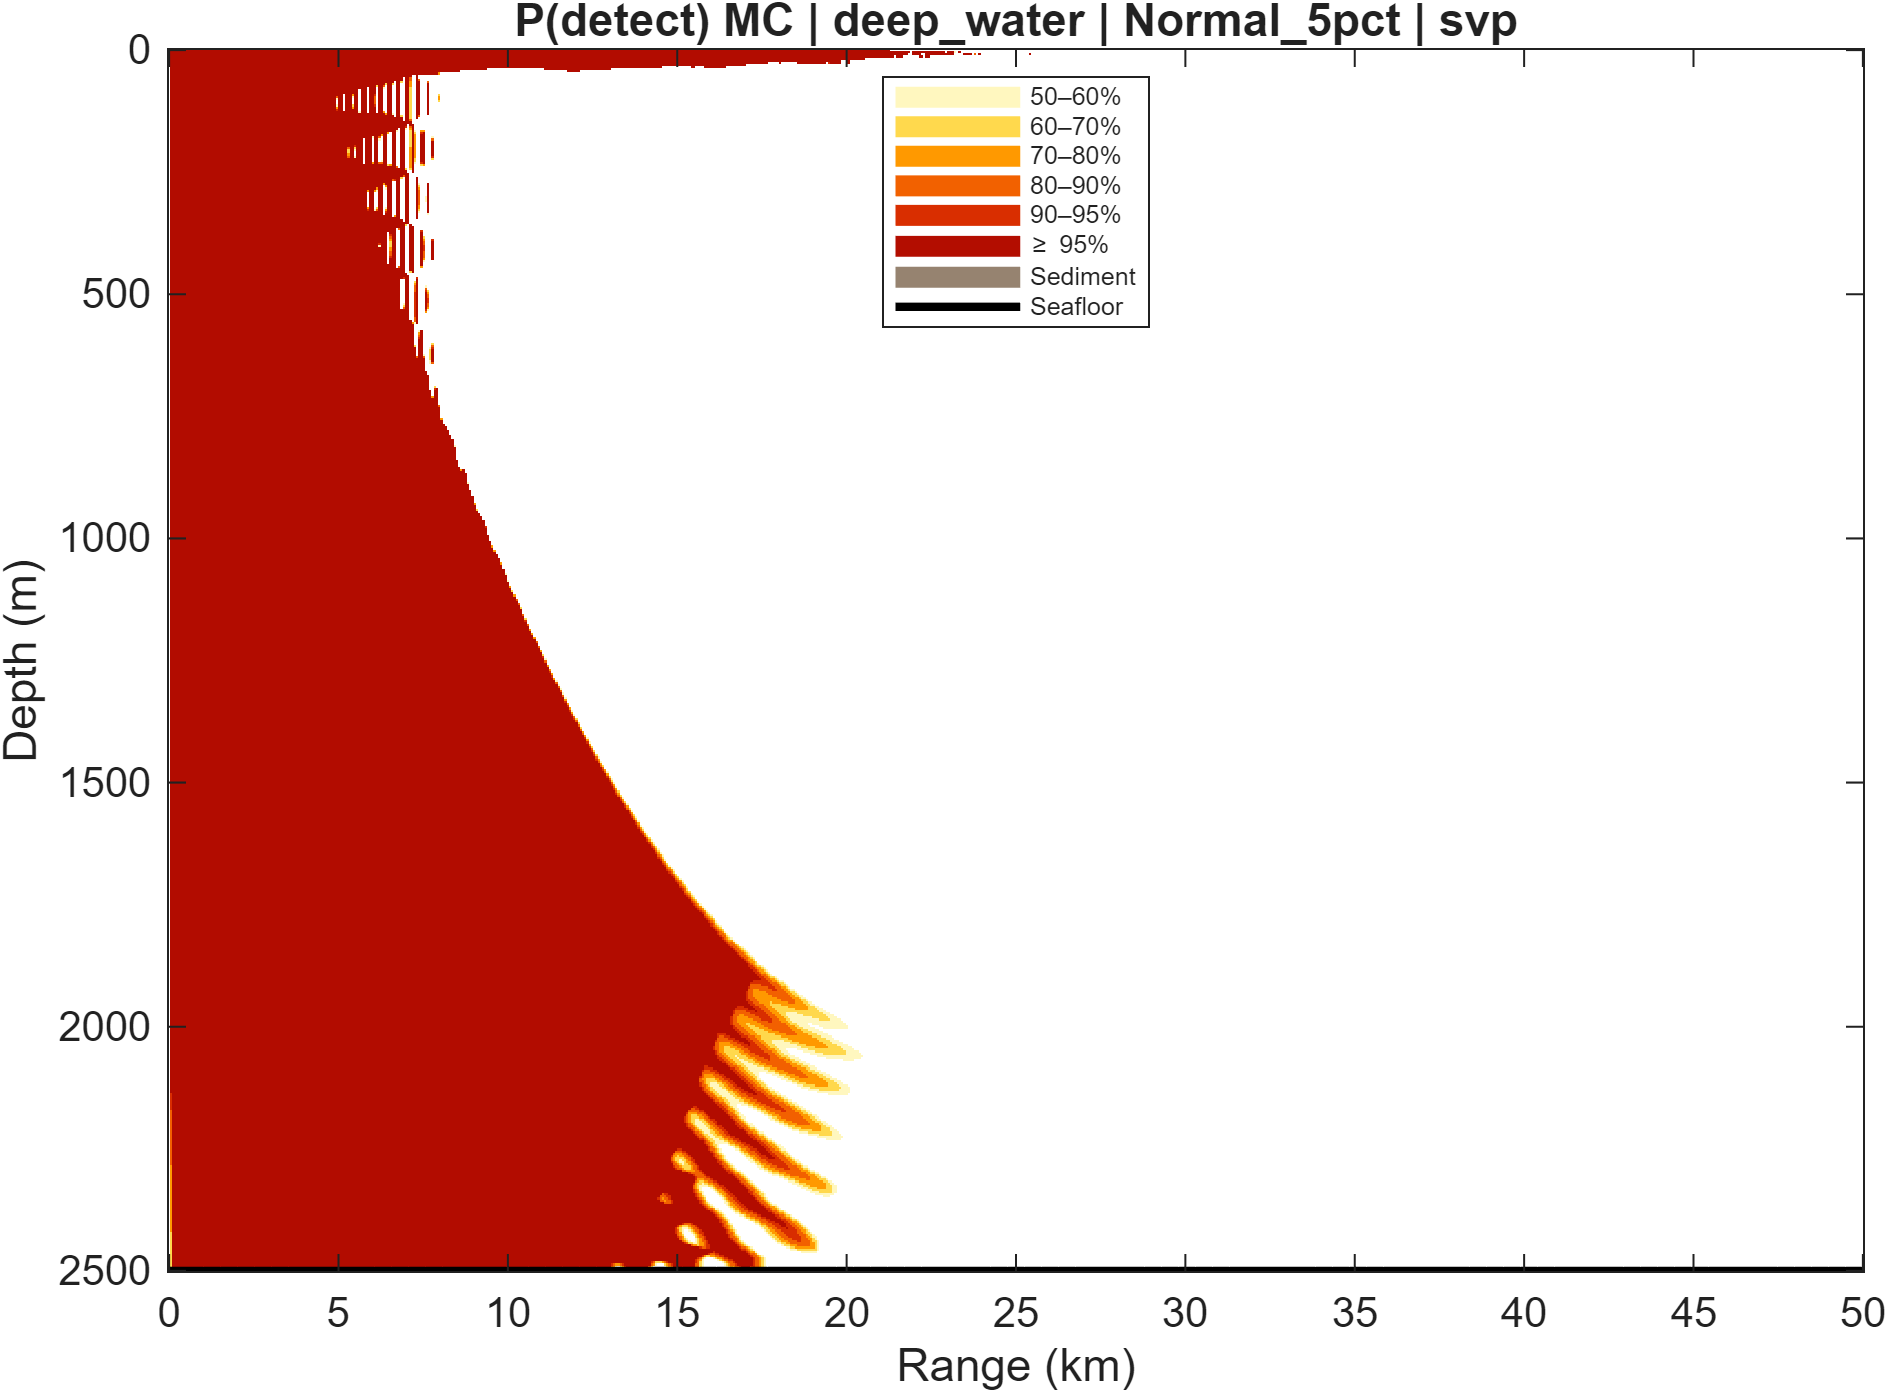
\includegraphics[width=\linewidth]{deep_water/Normal_5pct/figures/detect_empirical_svp.png}
    \caption{SVP}
  \end{subfigure}
  \caption{Detection failure probability $P_\mathrm{fail} = P(\TL > \mathrm{FOM})$
           for deep-water scenario, Normal\,5\%.
           The $z_S$ uncertainty (centre) produces broader shadow regions than
           frequency (left) or SVP (right), reflecting the stronger nonlinear
           sensitivity to source depth in deep water.}
  \label{fig:detect}
\end{figure}

% ============================================================
\section{Discussion}
\label{sec:discussion}

\subsection{Comparison with Prior Literature}

Finette~\cite{finette2009} reported PCE convergence at orders $K{=}2$--4 for
one-dimensional acoustic propagation with frequency and SVP uncertainty,
consistent with our deep-water freq and SVP results ($K^*{=}3$--6).
The non-convergence of $z_S$ at $K \leq 10$ was not observed in that study,
likely because the waveguide geometry considered does not exhibit the same
depth-dependent caustic structures as the Bellhop environments tested here.

Dosso et al.~\cite{jmse2022} compared MC and Delta methods for range-dependent
scenarios and found Delta accurate to within 5--10\% for $\leq2\%$ environmental
perturbations, consistent with our findings for the flat scenarios at Normal\,1\%.

\subsection{The $z_S$ Nonlinearity}

The persistent PCE non-convergence for $z_S$ in deep water is a physically
meaningful result.
In deep-water environments, the source depth relative to the sound-speed
minimum determines how many rays escape upward into the surface-reflected
path versus are trapped in the deep-sound-channel (SOFAR).
Near the channel axis, small changes in $z_S$ cause large, highly nonlinear
jumps in the modal excitation coefficients $\psi_m(z_S)$, producing TL
variations that are not well approximated by any finite polynomial.
This implies that any surrogate model (not just PCE) will struggle with $z_S$
uncertainty in deep-water scenarios; full MC is the only robust approach.

\subsection{LN3 and the MLE Problem}

Method-of-moments fitting is suboptimal compared to MLE.
However, MLE is not applicable to LHS samples because the LHS stratification
creates negative inter-sample correlation that invalidates the standard
i.i.d.\ log-likelihood~\cite{iman2008}.
A design-weighted pseudo-likelihood or copula-based correction would be required
for rigorous MLE; this remains an open methodological direction.

% ============================================================
\section{Conclusion}
\label{sec:conclusion}

We have presented a systematic UQ study of underwater acoustic TL using
Bellhop ray tracing across five propagation scenarios and three uncertainty
levels.
The Bellhop Finite-Difference Jacobian is validated against the closed-form
waveguide solution to $<5\%$ $L_1$ error, establishing the Bellhop-FD
Delta method as a mathematically rigorous approximation tool.

The principal findings are:
\begin{enumerate}
  \item \textbf{Bellhop-FD Delta}: reliable for flat bathymetry at $\leq1\%$
        perturbation.
        The 2nd-order Hessian correction exceeds 96\% of total variance at 5\%,
        signalling Taylor-series divergence.
        Slope bathymetry always requires a higher-order method.
  \item \textbf{PCE with LOO-CV}: converges for frequency and SVP at
        $K^* = 3$--6 with zero additional Bellhop runs.
        Source depth $z_S$ does not converge at any $K \leq 10$ in deep water ---
        a new finding attributable to modal excitation nonlinearity near the SOFAR channel.
  \item \textbf{LN3}: practically useful ($D_\mathrm{KS} < 0.17$) but formally
        rejected by the large-$N$ KS test.
        Method-of-moments fitting is the only consistent estimator for LHS samples.
  \item \textbf{MC}: the only reliable method for slope bathymetry and $z_S$
        uncertainty at $\geq5\%$ perturbation.
        $N = 300$ suffices for variance convergence; $N = 1000$ provides robust
        tail estimates for $P_\mathrm{fail}$.
\end{enumerate}

\textbf{Recommendation for operational use:}
Apply PCE-$K^*$ for flat-bottom scenarios with freq/SVP uncertainty.
Fall back to MC for slope environments, for $z_S$ uncertainty at $\geq5\%$,
or whenever the 2nd-order Hessian correction exceeds 50\% of total variance.
Report $P_\mathrm{fail}$ and P95 maps rather than variance alone to correctly
capture the directional character of acoustic uncertainty.

% ============================================================
\bibliographystyle{IEEEtran}
\bibliography{references}

\end{document}
